
%%%%%%%%%%%%%%%%%%%%%%%%%%%%%%%%%%%%%%%%%%%%%%%%%%%%%%%%%%%%%%%%%%%%%%%%%%%%%%%
%
%  EGSnrc beamdp utility manual
%  Copyright (C) 2015 National Research Council Canada
%
%  This file is part of EGSnrc.
%
%  EGSnrc is free software: you can redistribute it and/or modify it under
%  the terms of the GNU Affero General Public License as published by the
%  Free Software Foundation, either version 3 of the License, or (at your
%  option) any later version.
%
%  EGSnrc is distributed in the hope that it will be useful, but WITHOUT ANY
%  WARRANTY; without even the implied warranty of MERCHANTABILITY or FITNESS
%  FOR A PARTICULAR PURPOSE.  See the GNU Affero General Public License for
%  more details.
%
%  You should have received a copy of the GNU Affero General Public License
%  along with EGSnrc. If not, see <http://www.gnu.org/licenses/>.
%
%%%%%%%%%%%%%%%%%%%%%%%%%%%%%%%%%%%%%%%%%%%%%%%%%%%%%%%%%%%%%%%%%%%%%%%%%%%%%%%
%
%  Authors:         Charlie Ma, 1995
%                   Dave Rogers, 1995
%
%  Contributors:    Andrew Booth
%                   Blake Walters
%                   Iwan Kawrakow
%
%%%%%%%%%%%%%%%%%%%%%%%%%%%%%%%%%%%%%%%%%%%%%%%%%%%%%%%%%%%%%%%%%%%%%%%%%%%%%%%


\documentclass[12pt,twoside]{article}
\setlength{\textwidth}{6.5in}
\setlength{\textheight}{9.5in}
\setlength{\oddsidemargin}{0.0in}
\setlength{\evensidemargin}{0.0in}
\setlength{\topmargin}{-0.8in}
\setlength{\parindent}{0em}
\setlength{\topsep}{0ex}
\setlength{\itemsep}{0ex}

\newcommand{\Co}{$^{60}$Co}
\newcommand{\parsp}{~\hspace*{1.5em}}
\setlength{\parskip}{0.1in}
\setlength{\baselineskip}{0.4in}
\newcommand{\head}[1]{\begin{center}\begin{Large}{\bf #1}
                                              \end{Large}\end{center}}
\newcommand{\cen}[1]{\begin{center} #1 \end{center}                   }
\newcommand{\etal}{{\em et.al.}}
\newcommand{\etc}{{\em etc}}
\newcommand{\eg}{{\em e.g.}}
\newcommand{\ie}{{\em i.e.}}

\renewcommand{\refname}{}

\usepackage{html}

\usepackage{graphicx}

\usepackage{fancyhdr}
\renewcommand{\footrulewidth}{0.4pt}
\renewcommand{\headrulewidth}{0.4pt}


\lhead[\thepage~]{NRCC Report PIRS-0509(E)revA~-~printed \today}
\rhead[BEAMDP as a General-Purpose Utility]{~\thepage}
\rfoot{{\rightmark}}
\lfoot{{\leftmark}}
\cfoot{}

\begin{document}

\pagestyle{empty}
\begin{htmlonly}
For information about the authors and/or institutions involved with this
work, use the links provided in the author list.\\
\begin{rawhtml}
<br><br>
\end{rawhtml}
\begin{rawhtml}
<br><br>
\end{rawhtml}
\begin{rawhtml}
<br><br>
\end{rawhtml}

Use the Up button to get back to this page from within the document.
\begin{rawhtml}
<BR> <HR> <P>
\end{rawhtml}
\copyright Copyright 2015, National Research Council of
Canada Ottawa
\begin{rawhtml}
<BR> <HR> <P>
\end{rawhtml}
\end{htmlonly}

%\markright{BEAMDP as a General-Purpose Utility~~~~~~last edited 03 Nov 1999
%~~~~printed \today \hfill page~~}

%\markboth{BEAMDP as a General-Purpose Utility}{NRCC Report PIRS-0509(E)}

%\setcounter{page}{1}

\pagestyle{empty}
\title{BEAMDP as a General-Purpose Utility}
\author{ C.-M. Ma and D.W.O. Rogers \\
Ionizing Radiation Standards\\
National Research Council of Canada,
Ottawa\\
}
\date{Printed: \today \\
NRCC Report PIRS-0509(E)revA
\begin{latexonly}
\\
\end{latexonly}
}
\maketitle
\pagestyle{empty}

\pagenumbering{arabic}

\begin{center}
\begin{Large}
{\bf Abstract}
\end{Large}
\end{center}
BEAMDP (BEAM Data Processor) is developed for the OMEGA (Ottawa Madison
Electron Gamma Algorithm) project. This program can be used to analyze the
phase-space parameters of a clinical electron beam generated using
BEAMnrc and to derive the data required by a multiple-source model for
representation and reconstruction of the electron beam for use in Monte
Carlo radiotherapy treatment planning.


This report covers general BEAMDP inputs and outputs for deriving particle
energy spectral, mean energy, planar fluence and angular distributions.
It   describes how to combine phase-space data files and list particle
parameters on the screen,  and gives information on how to compile and run
BEAMDP.

\newpage
\mbox{}
\newpage

\setcounter{page}{1}
\pagestyle{fancy}
\tableofcontents

\newpage

\section{Introduction}

\noindent
BEAMDP (BEAM Data Processor) is a program,
originally developed for the OMEGA (Ottawa
Madison Electron Gamma Algorithm) project, to analyze the BEAM phase-space
data and to derive the spectral and planar fluence distributions for use
by beam characterization models (see BEAMDP users' manual). However,
BEAMDP can also be used as a utility program to derive other information
about the simulated electron beams from their phase-space files.

\noindent
When running BEAMDP, a user is given the following options:

\begin{enumerate}
\item to analyze a phase-space data file for beam characterization models.
When this option is chosen the user will be requested to provide further
information about the operation to be carried out (see BEAMDP users
manual);

\item to derive fluence vs position from a phase-space data file;

\item to derive energy fluence vs position from a phase-space data file;

\item to derive spectral distributions from a phase-space data file;

\item to derive energy fluence distributions from a phase-space data file;

\item to derive mean energy distributions from a phase-space data file;

\item to derive angular distributions from a phase-space data file;

\item to derive ZLAST distributions from a phase-space data file;

\item to derive the particle weight distribution from a phase-space file;

\item to derive an X-Y scatter plot of particles from a phase-space file;

\item to combine two phase-space files into one;

\item to list the paramenters of phase-space particles on the screen.
\end{enumerate}

\noindent
In the following sections we describe how options items 2-11 are
performed with BEAMDP. The details of beam characterization models and
their data processing procedures with BEAMDP can be found in BEAMDP user's
Manual.

\section{Methods}

\subsection{Definition of Scoring Quantities}

\begin{enumerate}
\item {\bf Fluence vs Position}: the total number of particles scored in
spatial bins of equal area. The user has a choice to score either planar
fluence, which does not take into account the angle at which the particle
strikes the scoring plane, or actual fluence (See section~\ref{fluencetype1}
below for more details on fluence type).;

\item {\bf Energy Fluence vs Position}: the total energy scored in spatial
bins of equal area.  Obtained by multiplying each particle's weight by it's
kinetic energy before scoring it in a bin. The user has a choice to score
either planar fluence or actual fluence (See section~\ref{fluencetype2} below);

\item {\bf Spectrum}: fluence (planar or actual--See section~\ref{fluencetype3})
scored in a user-specified
field vs energy with energy bins
of equal bin width within a specified spatial region.  Fluence is
normalized to the bin width and the number of incident particles;

\item {\bf Energy Fluence Distribution}: energy fluence
(planar or actual--See section~\ref{fluencetype4})
scored in a user-specified field vs
energy with energy bins
of equal bin width within a specified spatial region.  Fluence is
normalized to the bin width and the number of incident particles;


\item {\bf Mean Energy}: the ratio of the total particle energy to the
total number of particles scored in a spatial bin of equal area;

\item {\bf Angular Distribution}: the total number of particles scored in
an angular bin of equal bin width within a specified spatial region;

\item {\bf ZLAST Distribution}: the total number of particles scored in a
bin of equal bin width within a specified spatial region;

\item {\bf Weight Distribution}: number of particles vs the statistical
weight of particles with weight bins of equal width on a logarithmic
scale;

\item {\bf X-Y Scatter Plot}: a plot of the X-Y positions of all particles
having a user-specified charge and latch setting within a user-specified
field;

\item {\bf Statistics}: the error bars represent one-standard deviation
statistical uncertainties of the scored quantity.

\end{enumerate}

\subsection{Descriptions of Input Variables}

When running BEAMDP a user is requested to input information
regarding the distributions required, such as field types, field
dimensions, particle type, \verb+LATCH+ options, graph options, etc. This
section describes these input variables.

\noindent
In fact, BEAMDP provides two levels of prompts for information, one for
``experienced'' users and one for ``new'' users. Detailed descriptions of
the required input and range of acceptable values are given to the new
users. After the first run through the program the shorter, less
informative prompts are provided, to the ``experienced'' users. However,
at any time the user may obtain additional information about any of the
inputs by typing ``?'', or by providing an unacceptable value except for the
cases where the user is requested to input a filename (in this case press
Ctrl/C to interrupt the program).

\noindent
\subsubsection{field types:}

\noindent
Different field types have been used for planar fluence, spectrum, mean
energy and angular distributions and X-Y scatter plots
(see Figs.~\ref{fig-field-flu} and
\ref{fig-field-spe}). Detailed information can be found in each of the
sections describing the scoring quantities.

\begin{figure}[htbp]
\begin{center}
\vspace*{1cm}
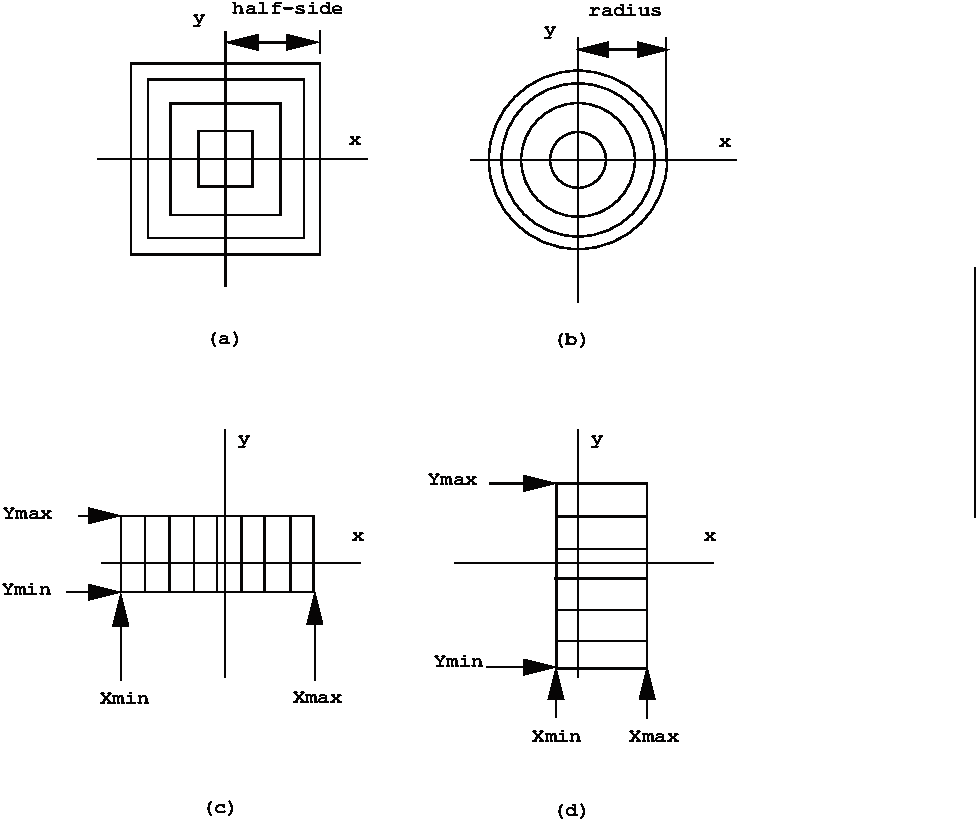
\includegraphics[height=19cm]{figures/field-flu}
\caption[]
{Field types for scoring planar fluence and mean energy: (a) square rings
of equal area; (b) annular bins of equal area; (c) rectangular bins
of equal area along x-axis; and (d) rectangular bins of equal
area along y-axis. }
\label{fig-field-flu}
\end{center}
\end{figure}

\begin{figure}[htbp]
\begin{center}
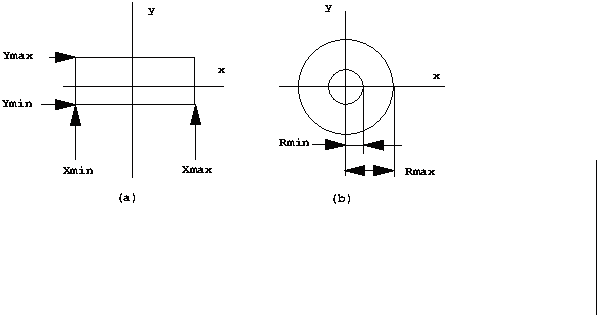
\includegraphics[height=10cm]{figures/field-spe}
\caption[]
{Field types for scoring spectrum, angular distribution and X-Y scatter plots:
(a) rectangular field and (b) annular field. }
\label{fig-field-spe}
\end{center}
\end{figure}

\noindent
\subsubsection{particle types:}

\noindent
One can choose from the following combinations:


IQ = -1 for electrons

IQ = ~0 for photons

IQ = ~1 for positrons

IQ = ~2 for all the particles

IQ = ~3 for electrons and positrons

\noindent
\subsubsection{LATCH filters:}

\noindent
\verb+LATCH+ is a phase-space parameter used to record the history of a
particle (see BEAMnrc user's manual). For example, if one has chosen
\verb+LATCH+ option 2 for the BEAM simulation,  bit 0 of \verb+LATCH+ is
used to indicate whether this particle is a photon or a charged particle
created by a photon (set to 1 if yes). Bits 1 - 23 of \verb+LATCH+ will be
used to record whether the particle has been to (IREGION-TO-BIT) regions 1
- 23 (each bit represents a region, i.e., bit 1 will be set to 1 if the
particle has been to/interacted in IREGION-TO-BIT region 1, and bit 5 will
be set to 1 if the particle has been to/interacted in IREGION-TO-BIT
region 5). Bits 24 - 28 will be used to record the number of an
(IREGION-TO-BIT) region where a secondary particle is created (it is
recorded as a 5-digit binary number). Thus, 00001 in bits 24 - 28 means
that the particle is created in IREGION-TO-BIT region 1, and 00101 in bits
24 - 28 means that the particle is created in IREGION-TO-BIT region 5.
Because a secondary can only be created in IREGION-TO-BIT regions 1 - 23,
if one finds 00000 in bits 24 - 28 of \verb+LATCH+, it indicates that the
particle is  a primary since any region not assigned a specific
IREGION-TO-BIT number is assigned a value of 23 by BEAM.  The
IREGION-TO-BIT region number, where a secondary is created, can be
calculated by $int(LATCH/2^{24})$.


\noindent
For data processing options 1-8, the user can ``filter" the particles output
by beamdp so that only
particles with certain \verb+LATCH+ bits set or not set will be output
for plotting.  There are 4 latch filters available, controlled by the setting
of the input variable {\tt I\_IN\_EX}.  A description of each filter, along
with the required input variables is given below:

\begin{description}
\item [{\tt I\_IN\_EX}=0] This is an inclusive/exclusive bit filter.  On the
same line as {\tt I\_IN\_EX}, the user must input the integers {\tt Nbit1} and
{\tt Nbit2}.  {\tt Nbit1} is the number of bits to include and {\tt Nbit2} is
the number of bits to exclude.  Restriction is that
0$\leq${\tt Nbit1}+{\tt Nbit2}$\leq$29.
Both {\tt Nbit1} and {\tt Nbit2} can be set to zero.  On the next line, the
user inputs {\tt BIT(I) (I=1,Nbit1)}, the bits to be included, and on
the following line {\tt BIT(I) (I=Nbit1+1,Nbit1+Nbit2)}, the bits to
be excluded.  If any of the first set of {\tt Nbit1} bits are set and none
of the second set of {\tt Nbit2} bits are set, the particle is scored.

\item [{\tt I\_IN\_EX}=1] This is an exclusive bit filter.  On the same line
as {\tt I\_IN\_EX}, the user has only to input the integer {\tt Nbit1}, the
number of bits to be excluded (0$\leq${\tt Nbit1}$\leq$29).  {\tt Nbit2} is
not relevant for this filter and is automatically set to 0.  On the
next line, the user inputs, {\tt BIT(I) (I=1,Nbit1)}, the bits to
be excluded.  If any of these {\tt Nbit1} bits are set, the particle
is NOT scored.

\item [{\tt I\_IN\_EX}=2] An inclusive region-of-origin filter.
The user inputs {\tt Nbit1} on the same line
as {\tt I\_IN\_EX}, where {\tt Nbit1} is the number of regions of origin
to be included.  Since regions of origin are distinguished only by their
values of {\tt IREGION\_TO\_BIT}, {\tt Nbit1} can also be seen as the
number of distinct values of {\tt IREGION\_TO\_BIT} to be included. The
restriction on {\tt Nbit1} is 0$\leq${\tt Nbit1}$\leq$24.  {\tt Nbit2} is
not relevant for this filter and is automatically set to 0.  On the
next line, the user inputs {\tt IREGION\_TO\_BIT(I) (I=1,Nbit1)}, the
{\tt IREGION\_TO\_BIT} values of the {\tt Nbit1} regions of origin to
be included.  If the particle originated in any one of these {\tt Nbit1}
regions, then it is scored.  Primary particles will be included if
{\tt IREGION\_TO\_BIT=0} is one of the {\tt Nbit1} values of
{\tt IREGION\_TO\_BIT} to include.

\item [{\tt I\_IN\_EX}=3] An exclusive region-of-origin filter.
The user inputs {\tt Nbit1} (0$\leq${\tt Nbit1}$\leq$24), the number of
regions of origin to be excluded, on the same line as {\tt I\_IN\_EX} and
ignores {\tt Nbit2}, since it is not relevant for this filter.  On the
next line the user inputs {\tt IREGION\_TO\_BIT(I) (I=1,Nbit1)}, the
{\tt IREGION\_TO\_BIT} values of the regions of origin to be excluded.
If a particle originated in any one of these regions, then it is NOT
scored.  Note that primary particles will be excluded if
{\tt IREGION\_TO\_BIT=0} is one of the {\tt Nbit1} values of
{\tt IREGION\_TO\_BIT} to exclude.

\end{description}

\noindent
\subsubsection{graph types:}
One can choose either normal-point graphs or histograms, except for the X-Y
scatter plots, which, by definition, are unconnected points in the X-Y plane.

\noindent
\subsubsection{fluence type:}
For fluence/energy fluence vs position and energy/energy fluence distributions,
the user can choose between plotting planar fluence or actual fluence.

\subsubsection{format of output data:}
All output graphics are in a format suitable for use by the \verb+xvgr+ plotting
package. If the user has another plotting package only the subroutine
``xvgrplot'' need be rewritten to match the needed format.

\subsubsection{file name inputs:}
File names should be given with extension. For example, for a phase-space
file scored at the first scoring plane during a BEAM simulation it can be
"try.egsphsp1". BEAMDP will check the first record of the file and
recognize whether it is a "MODE0" or a "MODE2" file (see BEAM user's
manual).  For the \verb+xvgr+ data file the extension can be arbitrary
although we find it useful to always call it \verb+ .xvgr+.

\subsubsection{multiple-curves:}
One can derive several planar fluence, mean energy, spectral and angular
distributions, and X-Y scatter plots from the same phase-space data and
output them into the same \verb+xvgr+ data file.

\subsection{Analysis of Statistical Uncertainties}

BEAMDP can be used as a BEAM utility program to analyze the phase-space
data and generate formatted data files suitable for \verb+xvgr+ plots.
Currently, one can derive either fluence, spectrum, mean energy, or
angular distributions from the phase-space data using BEAMDP.  The
statistical uncertainties on the derived distributions will depend on the
size of the phase-space data.\\

BEAMnrc uses the history-by-history method\cite{Wa02a} for estimating
uncertainty in scored quantities (eg dose, fluence).  In this method,
particles from each statistically independent event (ie each primary history)
are grouped together for uncertainty analysis.  Grouping is facilitated
by the negative energy markers in the phase space file\cite{Ro04a} which
mark the first particle scored for each primary history.  The history-by-history
method ensures that correlations between scored particles arising from the
same primary history are taken into account when calculating uncertainty.

Note that, until recently, BEAMDP assumed that each particle in the phase
space file represented a statistically-independent event.  It has
been shown\cite{Wa02a} that this does not result in a significant
underestimate of uncertainty even with the relatively high bremsstrahlung
splitting numbers used by the selective bremsstrahlung splitting (SBS)
algorithm in BEAM\cite{Ro04a}.  With the advent of the more efficient
directional bremsstrahlung splitting (DBS) algorithm\cite{Ka04a} in BEAM,
however,
splitting numbers have increased by as much as an order of magnitude,
potentially making
correlations a significant factor in uncertainty analysis.

The following
sections give detailed descriptions of the
formulas used in BEAMDP for determining uncertainties.
Most of
these equations are taken directly from the paper on history-by-history
statistics\cite{Wa02a}.

\subsubsection{ Basic Formulas }

BEAMDP reads the parameters of the phase-space particles and bins
particles
according to their position (for fluence distribution),
energy (for spectral distrubution), angle (for angular distribution), etc.
Within a bin, particles are grouped according to primary history.
Assuming that a
phase-space data file contains particles from $N$ primary histories,
the mean of a quantity of interest in a bin, ${\bf X}$ (${\bf X}$ can be
energy, angle, fluence, etc), can be calculated as
\begin{eqnarray}
\overline{X}& =&  \frac{\sum_{i=1}^{N}X_i}{N}
\end{eqnarray}
where $X_i$ is the sum of the contributions from the i-th primary history.
For most quantities of interest $X_i$ is the sum of the particle weights from
the i-th primary history.  However, if you are plotting energy fluence
or energy fluence vs position then $X_i$ is the sum of
(particle weight)*(particle energy), and
if you are plotting a distribution of particle weights then
each particle contributes unity to $X_i$ regardless of its weight.

The uncertainty in $\overline{X}$ is calculated using:
\begin{eqnarray}
s_{\overline{X}}& =& \sqrt{\frac{1}{N-1}\left(\frac{\sum_{i=1}^{N}X_i^2}
          {N}-\left(\frac{\sum_{i=1}^{N}X_i}{N}\right)^2\right)}
\label{sdeq}
\end{eqnarray}

Mean energy vs position presents a special case in BEAMDP
because mean energy is a ratio of correlated quantities.  The mean
energy in a bin, $\overline{E}$ is given by:
\begin{eqnarray}
\overline{E}& =&  \frac{\sum_{i=1}^{N}\left(wtE\right)_i}{\sum_{i=1}^{N}wt_i}
\end{eqnarray}
where $\left(wtE\right)_i$ is the sum of (particle weight)*(particle energy)
from the i-th primary history and $wt_i$ is the sum of particle weights from
the i-th primary history.  These are correlated
quantities that, if
output separately (as energy fluence vs position and fluence vs position,
respectively), would have their own uncertainties.

The fractional uncertainty in $\overline{E}$ is given by:
\begin{eqnarray}
\frac{s_{\overline{E}}}{\overline{E}}& =& \sqrt{\left({\frac{s_{\overline{
\left(wtE\right)}}}
{\overline{\left(wtE\right)}}}\right)^2 + \left({\frac{s_{\overline{wt}}}{\overline{wt}}}
\right)^2 -
\frac{2cov\left(wtE,wt\right)}{\left(N-1\right)
\overline{\left(wtE\right)}~\overline{wt}}}
\label{sdcoveqn}
\end{eqnarray}
where $s_{\overline{\left(wtE\right)}}$ is the uncertainty on
$\left(wtE\right)$ (or energy fluence vs position) and
$s_{\overline{wt}}$ is the uncertainty on $wt$ (or fluence vs position) and
are calculated using Equation~\ref{sdeq}, and $cov\left(wtE,wt\right)$
is the covariance of the two quantities, given by:
\begin{eqnarray}
cov\left(wtE,wt\right)& =&\frac{\sum_{i=1}^{N}
\left(wtE\right)_iwt_i}{N}-
\frac{\sum_{i=1}^{N}\left(wtE\right)_i\sum_{i=1}^{N}wt_i}{N^2}
\label{coveqn}
\end{eqnarray}

In practice, the calculation of covariance using Equation~\ref{coveqn} is
not valid if there are a small number of particles in a spatial bin.
We have set the minimum number of particles for considering covariance
in a bin to 10.  Thus, if there are $<$10 particles in the bin, then
$cov\left(wtE,wt\right)$ is set to 0.  This is consistent with the
calculation of uncertainty on ratios of correlated quantities in the BEAM
code.  In order to keep track of the number of particles in a spatial bin
BEAMDP uses an array called {\tt JUSTONE(I)} which is incremented every
time a particle contributes to bin {\tt I}.

For more details on calculating uncertainty and how we keep track of
$\sum_{i=1}^{N}X_i$ and $\sum_{i=1}^{N}X_i^2$ in each bin on the fly,
see the paper on history by history statistics\cite{Wa02a}.

\section{BEAMDP Utility Options}
\subsection{Fluence vs Position from a Phase-Space File}

When this option is chosen BEAMDP will process the phase-space data and
generate a fluence vs position data file with format suitable for \verb+xvgr+ plots.
The user will be asked to select field types, field dimensions, particle
type, \verb+LATCH+ options, the names of the
phase-space file to be processed and the data file for outputs, the graph
type, and finally the type of fluence to be plotted.  Each data
point in the data file represents the total number of particles scored
within a given spatial bin for the particle types and \verb+LATCH+ options
chosen.

\subsubsection{Field Types:}
There are three field types for the planar fluence distributions:
\begin{enumerate}
\item a circular field with annular regions of equal area (the user should
input the number of annular regions requested and the field radius, see
Fig.~\ref{fig-field-flu}b);
\item a square field with square rings of equal area (the user should
input the number of spatial bins requested and the half-side of the square
field, see Fig.~\ref{fig-field-flu}a);
\item a rectangular field with equal spatial bins along x- or y-axis (the
user should input the number of bins requested, the orientation (0 - along
x-axis; 1 - along y-xis), and the x- and y-coordinates defining the field,
see Fig.~\ref{fig-field-flu} c and d); \end{enumerate}

\subsubsection{Fluence Types:}
\label{fluencetype1}
The fluence vs position option gives the user the choice of plotting
either planar fluence (1) or the actual fluence (0) as a function of
position.
Planar fluence plots the sum of the particle weights in each spatial
bin.  Actual fluence divides each particle weight by
MAX(0.08716, cos(particle angle wrt scoring plane)) before
adding it to the sum.  The number 0.08716 is cos(85$^o$) and is a lower limit
to prevent division by 0 for angles close to 90$^o$.

\subsection{Energy Fluence vs Position from a Phase-Space File}

When this option is chosen BEAMDP will process the phase-space data and
generate an energy fluence vs position data file with format suitable for \verb+xvgr+ plots.
The input parameters are the same as for a fluence vs position plot.

\subsubsection{Fluence Types:}
\label{fluencetype2}
Similar to fluence vs position, the user can choose to plot either planar
energy fluence (1) or actual energy fluence (0).  Planar energy fluence
plots the sum of the product (particle weight*kinetic energy) in each
spatial bin, while actual fluence divides the product by the cosine
of the particle's angle with respect to the scoring plane (again, there
is a cap of 85$^o$ to avoid division by zero).


\subsection{Energy Spectrum from a Phase-Space File}
When this option is chosen BEAMDP will process the phase-space data and
generate a spectral data file with format suitable for \verb+xvgr+ plots. The
user will be asked to select field types and field dimensions, energy
range, particle type, \verb+LATCH+ options, the
names of the phase-space file to be processed and the data file for
outputs graph options, graph type, and finally the fluence type.
Each data point in the data file represents the fluence
within a given energy bin for the particle types and
\verb+LATCH+ options chosen.  Fluence is normalized by the bin width,
number of incident particles and the area of the field being considered.

\subsubsection{Field Types:}

For spectral calculations one can choose the following field types:
\begin{enumerate}
\item a rectangular region anywhere on the scoring plane (the user should
input the  x- and y-coordinates defining the region, see
Fig.~\ref{fig-field-spe}a);

\item an annular region centred at beam axis (the user should input the
inner and outer radius for the annular region, see
Fig.~\ref{fig-field-spe}b); \end{enumerate}

\subsubsection{Range of Energy:}
The energies should be between 0 and the maximum energy of the particles
in the phase-space file.

\subsubsection{Fluence Types:}
\label{fluencetype3}
The energy spectrum option also allows the user to choose between plotting
planar fluence (1) and actual fluence (0) vs energy.  Planar fluence
sums the particle weights in each energy bin and divides the sum by the
number of incident particles, the area of the scoring region selected
by the user, and the width of the energy bins.  Actual fluence divides
each particle weight by
MAX(0.08716, cos(particle angle wrt scoring plane)) before adding
it to the sum in each energy bin.

\subsection{Energy Fluence Distribution from a Phase-Space File}
When this option is chosen BEAMDP will process the phase-space data and
generate an energy fluence vs energy distribution with format suitable for
\verb+xvgr+ plots.  Input parameters are the same as for the energy
distribution option.

\subsubsection{Fluence Types:}
\label{fluencetype4}
Similar to the energy distribution, the user can plot planar energy fluence (1) or
actual energy fluence (0) vs energy.  Planar fluence
sums the product (particle weight*kinetic energy) in each energy bin and
divides the sum by the
number of incident particles, the area of the scoring region selected
by the user, and the width of the energy bins.  Actual fluence divides
each product (particle weight*kinetic energy) by
MAX(0.08716, cos(particle angle wrt scoring plane)) before adding
it to the sum in each energy bin.

\subsection{Mean Energy from a Phase-Space File}

When this option is chosen BEAMDP will process the phase-space data and
generate a mean energy data file with format suitable for \verb+xvgr+ plots. The
user will be asked to select field types, field dimensions, particle type,
\verb+LATCH+ options, graph options, and finally the names of the phase-space
file to be processed and the data file for outputs.  Each data point in
the data file represents the mean energy of the particles scored within a
given spatial bin for the particle types and \verb+LATCH+ options chosen.

\subsubsection{Field Types:}

There are three field types for the planar fluence distributions:

\begin{enumerate}
\item a circular field with annular regions of equal area (the user should
input the number of annular regions requested and the field radius, see
Fig.~\ref{fig-field-flu}b);

\item a square field with square rings of equal area (the user should
input the number of spatial bins requested and the half-side of the square
field, see Fig.~\ref{fig-field-flu}a);

\item a rectangular field with equal spatial bins along x- or y-axis (the
user should input the number of bins requested, the orientation, and the
x- and y-coordinates defining the field, see Fig.~\ref{fig-field-flu} c
and d); \end{enumerate}

\subsection{Angular Distribution from a Phase-Space File}
When this option is chosen BEAMDP will process the phase-space data and
generate an angular data file with format suitable for XVGR/XMGR plots.
The user will be asked to select field types and field dimensions, angular
range, particle type, \verb+LATCH+ options, graph options, and finally the
names of the phase-space file to be processed and the data file for
outputs.  Each data point in the data file represents the total number of
particles scored within a given angular bin (the angle between the
particle incident direction and the z-axis) for the particle types and
\verb+LATCH+ options chosen.


\subsubsection{Field Types:}
For spectral calculations one can choose the following field types:
\begin{enumerate}
\item a rectangular region anywhere on the scoring plane (the user should
input the  x- and y-coordinates defining the region, see
Fig.~\ref{fig-field-spe}a);

\item an annular region centred at beam axis (the user should input the
inner and outer radius for the annular region, see
Fig.~\ref{fig-field-spe}b);

\end{enumerate}

\subsubsection{Range of Angle:}
The angles should be between 0 and 90 degrees.

\subsection{ZLAST Distribution from a Phase-Space File}
This option will process the phase-space data and generate a ZLAST data
file with format suitable for XVGR/XMGR plots. The user will be asked to
select field types and field dimensions, ZLAST range, particle type,
\verb+LATCH+ options, graph options, and finally the names of the
phase-space file to be processed and the data file for outputs.  Each data
point in the data file represents the total number of particles scored
within a given ZLAST bin (the z-position of the particle where it is
generated or last scattered) for the particle types and \verb+LATCH+
options chosen.


\subsubsection{Field Types:}

For ZLAST scoring one can choose the following field types:

\begin{enumerate}
\item a rectangular region anywhere on the scoring plane (the user should
input the  x- and y-coordinates defining the region, see
Fig.~\ref{fig-field-spe}a);

\item an annular region centred at beam axis (the user should input the
inner and outer radius for the annular region, see
Fig.~\ref{fig-field-spe}b); \end{enumerate}

\subsubsection{Range of ZLAST:}

This should be consistent with the simulation geometry (the default range
is 0 - 100 cm).

\subsection{Particle Weight Distribution from a Phase-Space File}

When this option is chosen, BEAMDP will generate a distribution of
particle weights which can be displayed using XMGR/XVGR.  The user
will be asked to input the
field type and field dimensions, particle type,
weight range, \verb+LATCH+ options, graph options,
the name of the phase-space file to be processed and the name of the output
file.  Each data point represents the number of particles, of the user-selected
type and \verb+LATCH+ properties, having weights
falling within a given energy bin.  Weight bins are of equal width on
a logarithmic scale to allow greater resolution of low weights.

\subsubsection{Field Types:}

Similar to the energy spectrum option (see above) the user can choose
either a rectangular field anywhere in the scoring plane or an annular field
centred on the Z-axis in which to determine particle weights.

\subsubsection{ Range of Particle Weights:}

The minimum particle weight chosen for plotting must be $>$ 0.

\subsection{X-Y Scatter Plot from a Phase-Space File}

This option generates a scatter plot of the X-Y positions of particles
in a user-specified field.  In addition to specifying the field type
(annular or rectangular) and dimensions, the user also specifies the
charge, energy range and latch settings of the particles to be plotted.
{\tt beamdp} will then output the X-Y positions of all particles meeting
the charge, energy and latch criteria in the specified field.

\subsubsection{Field Types:}

The user can specify either a rectangular field anywhere on the scoring plane or
an annular field centred on the Z-axis.  These field types are the same as
those available for the energy spectrum option (see above).

\subsubsection{Range of Energy:}
The minimum and maximum particle energies of the specified range
should be between 0 and the maximum energy of the particles in the
phase-space file.

\subsection{Combine two phase-space files into one}

This feature is useful to those who run BEAM on different machines (with
different random number seeds, of course) and would like to combine
separate phase-space data into one file.


It has been designed to read the phase-space data from file 1 and write it
to file 2. Note the two files must be of the same mode (either "MODE0" or
"MODE2"). After finishing reading/writing the phase-space data BEAMDP will
re-write the  first record of file 2 with proper numbers of the
particles/photons stored in the file and their minimum and maximum
energies, etc.

\subsection{ List paramenters of phase-space particles}
Another userful feature of BEAMDP is to list parameters of phase-space
particles on the screen. One can choose the number of particles to be
listed and the particle types (IQ = -1 for electrons, IQ = 0 for photons,
IQ = 1 for positrons, IQ = 2 for all the particle types, IQ = 3 for
charged particles). The name of the phase-space data file should be given
with proper extension (.egs4phsp1, .egs4phsp2 or .egs4phsp3).

\subsubsection{Parameters to Be Listed}

The following parameters are printed on the screen:
\begin{enumerate}
\item {\bf Energy}: particle energy (kinetic only) in MeV

\item {\bf IQ}: charge of particle (-1 for electron, 0 for photon, 1 for
positron)

\item {\bf X,Y}: x- and y-coordinates in cm

\item {\bf U,V,W}: direction cosines with respect to x-, y-, and z-axis

\item {\bf WEIGHT}: weight of particle

\item {\bf LATCH}: a tag to record the history of a particle. Only bits 0
- 28 will be listed (bits 29 - 31 have been used by BEAM to store particle
charge and another parameter NPASS, see ``BEAM Users Manual'' (1995)).
\end{enumerate}

\subsubsection{ A Sample Listing}
The following is a listing for an electron created in (IREGION-TO-BIT)
region 7 and has gone through regions 7, 1 (note, because of the way in
which the user has set up the IREGION-TO-BIT numbers, higher region numbers
mean that the regions are further away from the scoring plane). It can be
seen that bits 14 and 21 of \verb+LATCH+ are also set but this probably an
indication that its parent has gone through regions 14 and 21 because it
is very unlikely that an electron created in region 7 could go through
regions 14 and 21 and then scatter back to region 1 (see ``BEAM Users
Manual'' for more details).


\noindent
 ENERGY   ~IQ  ~~~X  ~~~~Y  ~~~~U      ~~~~~V      ~~~~~W     ~~~~WEIGHT       ~~~~~LATCH (set=1, not set=0)

\noindent
  ~~~~1.330 ~~~ -1   ~2.419   3.015  0.019  0.209  0.978  ~ 1.000E+00  ~00111 001000000100000010000010


\noindent
Note \verb+LATCH+ is given in 2 parts: each number (0 or 1) in the first part
represents a bit for \verb+LATCH+ bits 24-28 (where a secondary particle
was created), each number in the second part represents a bit for
\verb+LATCH+ bits 0-23 (where the particle has been).

Thus, one should read \verb+LATCH+ bits (in increasing order) from right
to left.


\section{Compile and Run BEAMDP}
BEAMDP is a stand alone program for BEAM data processing. In order to
output graphics data in a format for use by \verb+xmgrace+ plotting package
BEAMDP
uses a subroutine called xvgrplot (written by Andrew Booth). If a user has
another plotting package, subroutine xvgrplot can be modified to output in a
needed format.


The {\tt MORTRAN} BEAMDP source file, {\tt beamdp.mortran}, is stored in the
directory\\
\$OMEGA\_HOME/progs/beamdp together with its {\tt Makefile}.  This directory
also contains the files {\tt beammodel\_macros.mortran} and
{\tt beammodel\_routines.mortran} which are used by BEAMnrc\cite{Ro04a}
 and DOSXYZnrc\cite{WR04a} to implement multiple source models created
using BEAMDP (See the BEAMDP Manual\cite{MR04a} for more about multiple
source models).

\subsection{Compile BEAMDP}

BEAMDP is installed and compiled as part of the OMEGA/BEAM installation
(See the BEAMnrc Manual\cite{Ro04a} for installation instructions).

To compile BEAMDP separately, go into
{\tt \$OMEGA\_HOME/progs/beamdp} and issue the command\\
{\tt make}\\
This will concatenate the files specified in the variable
{\tt SOURCES} in {\tt Makefile} to create {\tt mortjob.mortran}
and then do the MORTRAN/Fortran compilation on this.
Note that {\tt Makefile} also references {\tt \$HEN\_HOUSE/specs/config.conf}
and {\tt \$HEN\_HOUSE/specs/beamnrc.spec}.

After compilation, the files {\tt beamdp\_config.mortlst} (MORTRAN listing)
and {\tt beamdp\_config.f} (Fortran code) will be left in
{\tt \$OMEGA\_HOME/progs/beamdp}, while the executable, {\tt beamdp*}, will
be copied to the {\tt \$HEN\_HOUSE/bin/config} directory for your
particular configuration.

\subsection{Run BEAMDP}
To run BEAMDP from the command line one can issue the command
(from any directory):
\begin{verbatim}
beamdp
\end{verbatim}
Note that you must have included the directory
{\tt \$HEN\_HOUSE/bin/config} in your
{\tt \$PATH} environment variable, where {\tt config} is the name
of the configuration you are running on (eg {\tt gcc}, {\tt win2k}).
BEAMDP will prompt for input.

Running BEAMDP is much easier with the BEAMDP GUI\cite{Tr04}.  The GUI enables you
to run different analyses of the same phase space data without having to
re-enter all parameters (such as field size/type, bit filters, etc).
Alternatively, you may run the same analysis on a different phase space
file simply by changing the name of the phase space file to analyze.

To run the BEAMD GUI from a Linux/Unix window, type:
\begin{verbatim}
beamdp_gui
\end{verbatim}
from any directory.  You
must have sourced the file {\tt beamnrc\_cshrc\_additions} (or\\
{\tt beamnrc\_bashrc\_additions}) in your {\tt .cshrc} (or {\tt .bashrc})
file (See the BEAMnrc User's Manual\cite{Ro04a} for more about this).

To run the GUI in a Windows environment, double click on the GUI icon
(or on the word {\tt beamdp\_gui} after using Windows Explorer to enter
directory {\tt \$OMEGA\_HOME/progs/gui/beamdp}).

\section{References}
\renewcommand{\rightmark}{References}
\vspace*{-1cm}
\setlength{\baselineskip}{0.5cm}
\bibliography{../irs}
\bibliographystyle{unsrt}


\end{document}
